\documentclass[letterpaper, 12pt]{article}
\textwidth=6.5in
\textheight=9.5in
\topmargin=-0.75in
\oddsidemargin=0.0in
\evensidemargin=0.0in

\usepackage{graphicx}
\usepackage{enumitem}
\usepackage{amssymb, amsmath}
\usepackage{xcolor}
\usepackage{listings}

\usepackage{times}
\usepackage{natbib}
\usepackage{etoolbox}
\usepackage{astjnlabbrev-jh}
\usepackage{bibentry}
\usepackage{ifthen}
\usepackage{epsfig}

\usepackage{commath}
\usepackage{rotating}

\usepackage{dirtree}
\usepackage{changepage}

% To allow .ps files
\usepackage{auto-pst-pdf}

% \lstset{
% language=Python,
% showstringspaces=false,
% formfeed=\newpage,
% tabsize=4,
% commentstyle=\itshape,
% basicstyle=\ttfamily,
% morekeywords={models, lambda, forms}
% }
 
% \newcommand{\code}[2]{
% \hrulefill
% \subsection*{#1}
% \lstinputlisting{#2}
% \vspace{2em}
% }

% Default fixed font does not support bold face
\DeclareFixedFont{\ttb}{T1}{txtt}{bx}{n}{10} % for bold
\DeclareFixedFont{\ttm}{T1}{txtt}{m}{n}{10}  % for normal
% twelve-sized ttm:
\DeclareFixedFont{\tttb}{T1}{txtt}{bx}{n}{12}  % for bold
\DeclareFixedFont{\tttm}{T1}{txtt}{m} {n}{12}  % for normal

\DeclareFixedFont{\ttnm}{T1}{txtt}{m}{n}{9.8}  % for normal

% Custom colors
\usepackage{color}
\definecolor{deepblue}  {rgb}{0.0, 0.0, 0.5}
\definecolor{deepred}   {rgb}{0.8, 0.0, 0.0}
\definecolor{deepgreen} {rgb}{0.0, 0.5, 0.0}
\definecolor{commentc}  {rgb}{0.5, 0.5, 0.5}
\definecolor{DodgerBlue}{rgb}{0.1, 0.6, 1.0}

% Python style for highlighting
\newcommand\pythonstyle{\lstset{
language=Python,
basicstyle = \ttm,
morekeywords = {self, as, assert, with, yield}, % Add keywords here
keywordstyle = \ttb\color{blue},       %
emph        = {MyClass, __init__},     % Custom highlighting
emphstyle   = \ttb\color{DodgerBlue},  % Custom  highlighting style
stringstyle = \color{deepred},         % Strings highlighting style
commentstyle=\color{commentc},         % Comment highlighting style
frame       = tb,                      % Any extra options here
showstringspaces = false
}}

% Python environment:
\lstnewenvironment{python}[1][]{\pythonstyle\lstset{#1}}{}
% Python for external files:
\newcommand\pythonexternal[2][]{{\pythonstyle\lstinputlisting[#1]{#2}}}
% Python for inline:
\newcommand\pythoninline[1]{{\pythonstyle\lstinline!#1!}}


% Python style for highlighting
\newcommand\plainstyle{\lstset{
language=Python,
basicstyle = \ttnm,
keywordstyle= \ttnm,                %
emph        = {MyClass, __init__},  % Custom highlighting
emphstyle   = \ttnm\color{black},   % Custom  highlighting style
stringstyle = \color{black},        % Strings highlighting style
commentstyle=\color{black},         % Comment highlighting style
frame       = tb,                   % Any extra options here
showstringspaces = false
}}

% Plain environment:
\lstnewenvironment{plain}[1][]{\plainstyle\lstset{#1}}{}

\newcommand\plaininline[1]{{\plainstyle\lstinline!#1!}}

% To use boldface verbatim:
%\lstset{basicstyle=\ttfamily,
%        escapeinside={||},
%        mathescape=true}

\lstset{
    language={[LaTeX]TeX},
    basicstyle=\tt\color{red},
    escapeinside={||},
}

\bibliographystyle{apj_hyperref}
\usepackage[%pdftex,      %%% hyper-references for pdflatex
bookmarks=true,           %%% generate bookmarks ...
bookmarksnumbered=true,   %%% ... with numbers
colorlinks=true,          % links are colored
citecolor=blue,           % green   % color of cite links
linkcolor=blue,           %cyan,         % color of hyperref links
menucolor=blue,           % color of Acrobat Reader menu buttons
urlcolor=blue,            % color of page of \url{...}
breaklinks=true,
linkbordercolor={0 0 1},  %%% blue frames around links
pdfborder={0 0 1},
frenchlinks=true]{hyperref}
%\usepackage{breakurl}

\newcommand{\eprint}[1]{\href{http://arxiv.org/abs/#1}{#1}}
\newcommand{\ISBN}[1]{\href{http://cosmologist.info/ISBN/#1}{ISBN: #1}}
\providecommand{\adsurl}[1]{\href{#1}{ADS}}

% hyper ref only the year in citations:
\makeatletter
% Patch case where name and year are separated by aysep:
\patchcmd{\NAT@citex}
  {\@citea\NAT@hyper@{%
     \NAT@nmfmt{\NAT@nm}%
     \hyper@natlinkbreak{\NAT@aysep\NAT@spacechar}{\@citeb\@extra@b@citeb}%
     \NAT@date}}
  {\@citea\NAT@nmfmt{\NAT@nm}%
   \NAT@aysep\NAT@spacechar\NAT@hyper@{\NAT@date}}{}{}
% Patch case where name and year are separated by opening bracket:
\patchcmd{\NAT@citex}
  {\@citea\NAT@hyper@{%
     \NAT@nmfmt{\NAT@nm}%
     \hyper@natlinkbreak{\NAT@spacechar\NAT@@open\if*#1*\else#1\NAT@spacechar\fi}%
       {\@citeb\@extra@b@citeb}%
     \NAT@date}}
  {\@citea\NAT@nmfmt{\NAT@nm}%
   \NAT@spacechar\NAT@@open\if*#1*\else#1\NAT@spacechar\fi\NAT@hyper@{\NAT@date}}
  {}{}
\makeatother


%\def\bibAnnoteFile#1{}
%\bibpunct[, ]{(}{)}{,}{a}{}{,}

% Packed reference list:
\setlength\bibsep{0pt}

% \pagestyle{myheadings}
% \markright{MC\sp{3}}
% \pagenumbering{arabic}


% :::::::::::::::::::::::
\newcommand\degree{\degr}
%\newcommand\degrees{\degree}
\newcommand\vs{\emph{vs.}}

% unslanted mu, for ``micro'' abbrev.
\DeclareSymbolFont{UPM}{U}{eur}{m}{n}
\DeclareMathSymbol{\umu}{0}{UPM}{"16}
\let\oldumu=\umu
\renewcommand\umu{\ifmmode\oldumu\else\math{\oldumu}\fi}
\newcommand\micro{\umu}
\newcommand\micron{\micro m}
\newcommand\microns{\micron}

\let\oldsim=\sim
\renewcommand\sim{\ifmmode\oldsim\else\math{\oldsim}\fi}
\let\oldpm=\pm
\renewcommand\pm{\ifmmode\oldpm\else\math{\oldpm}\fi}
\newcommand\by{\ifmmode\times\else\math{\times}\fi}
\newcommand\ttt[1]{10\sp{#1}}
\newcommand\tttt[1]{\by\ttt{#1}}
\newcommand\tablebox[1]{\begin{tabular}[t]{@{}l@{}}#1\end{tabular}}
\newbox{\wdbox}
\renewcommand\c{\setbox\wdbox=\hbox{,}\hspace{\wd\wdbox}}
\renewcommand\i{\setbox\wdbox=\hbox{i}\hspace{\wd\wdbox}}
\newcommand\n{\hspace{0.5em}}
\newcommand\marnote[1]{\marginpar{\raggedright\tiny\ttfamily\baselineskip=9pt #1}}
\newcommand\herenote[1]{{\bfseries #1}\typeout{======================> note on page \arabic{page} <====================}}
\newcommand\fillin{\herenote{fill in}}
\newcommand\fillref{\herenote{ref}}
\newcommand\findme[1]{\herenote{(FINDME: #1)}}

\newcount\timect
\newcount\hourct
\newcount\minct
\newcommand\now{\timect=\time \divide\timect by 60
         \hourct=\timect \multiply\hourct by 60
         \minct=\time \advance\minct by -\hourct
         \number\timect:\ifnum \minct < 10 0\fi\number\minct}

\newcommand\citeauthyear[1]{\citeauthor{#1} \citeyear{#1}}

\newcommand\mc{\multicolumn}
\newcommand\mctc{\multicolumn{2}{c}}


% {\tttm -h, --help} \\
% Print the list of arguments. \newline

% \newenvironment{myindentpar}[1]%
%   {\begin{list}{}%
%          {\setlength{\leftmargin}{3cm}}%
%      \item[]%
%   }
% {\end{list}}

\newenvironment{packed_enum}{
\begin{enumerate}[leftmargin=3cm]
   \setlength{\itemsep}{1pt}
   \setlength{\parskip}{5pt}
   \setlength{\parsep}{0pt}
}{\end{enumerate}}

\newcommand{\argument}[2]{{\noindent\tttm #1}%
\begin{adjustwidth}{2.5em}{0pt}%
#2 \vspace{0.3cm}%
\end{adjustwidth}%
}

%\newcommand{\ttmb}[1]{\tttm\color{#1}}
\newcommand{\routine}[2]{{\noindent\tttm\color{blue} #1:}%
\begin{adjustwidth}{2.0em}{0pt}%
#2 \vspace{0.15cm}%
\end{adjustwidth}%
}

% \newcommand{\routine}[2]{{\noindent\tttm\color{blue} #1}%
% \begin{adjustwidth}{0.0em}{0pt}%
%  #2 \vspace{0.15cm}%
% \end{adjustwidth}%
% }

% :::::::::::::::::: jhmacs2.tex :::::::::::::::::::::::::::::::::::::
\typeout{Joe Harrington's personal setup, Wed Jun 17 10:53:17 EDT 1998}
% Tue Mar 29 22:23:03 EST 1994

% :::::: pato.tex ::::::
% Joetex character unreservations.
% This file frees most of TeX's reserved characters, and provides
% several alternatives for their functions.


% utility
\catcode`@=11

% comments are first....
\newcommand\comment[1]{}

\newcommand\commenton{\catcode`\%=14}
\newcommand\commentoff{\catcode`\%=12}

% Not-a-comment:
\newcommand\nocomment[1]{#1}

\renewcommand\math[1]{$#1$}
\newcommand\mathshifton{\catcode`\$=3}
\newcommand\mathshiftoff{\catcode`\$=12}

\comment{alignment tab}
\let\atab=&
\newcommand\atabon{\catcode`\&=4}
\newcommand\ataboff{\catcode`\&=12}

\let\oldmsp=\sp
\let\oldmsb=\sb
\def\sp#1{\ifmmode
           \oldmsp{#1}%
         \else\strut\raise.85ex\hbox{\scriptsize #1}\fi}
\def\sb#1{\ifmmode
           \oldmsb{#1}%
         \else\strut\raise-.54ex\hbox{\scriptsize #1}\fi}
\newbox\@sp
\newbox\@sb
\def\sbp#1#2{\ifmmode%
           \oldmsb{#1}\oldmsp{#2}%
         \else
           \setbox\@sb=\hbox{\sb{#1}}%
           \setbox\@sp=\hbox{\sp{#2}}%
           \rlap{\copy\@sb}\copy\@sp
           \ifdim \wd\@sb >\wd\@sp
             \hskip -\wd\@sp \hskip \wd\@sb
           \fi
        \fi}
\def\msp#1{\ifmmode
           \oldmsp{#1}
         \else \math{\oldmsp{#1}}\fi}
\def\msb#1{\ifmmode
           \oldmsb{#1}
         \else \math{\oldmsb{#1}}\fi}
\def\supon{\catcode`\^=7}
\def\supoff{\catcode`\^=12}
\def\subon{\catcode`\_=8}
\def\suboff{\catcode`\_=12}
\def\supsubon{\supon \subon}
\def\supsuboff{\supoff \suboff}


\newcommand\actcharon{\catcode`\~=13}
\newcommand\actcharoff{\catcode`\~=12}

\newcommand\paramon{\catcode`\#=6}
\newcommand\paramoff{\catcode`\#=12}

\comment{And now to turn us totally on and off...}

\newcommand\reservedcharson{ \commenton  \mathshifton  \atabon  \supsubon
                             \actcharon  \paramon}

\newcommand\reservedcharsoff{\commentoff \mathshiftoff \ataboff \supsuboff
                             \actcharoff \paramoff}

\newcommand\nojoe[1]{\reservedcharson #1 \reservedcharsoff}

\catcode`@=12
\reservedcharsoff

\reservedcharson
\newcommand\jhauth[1]{{#1}}
\newcommand\jhstud[1]{{#1}}

\comment{Must have ONLY ONE of these... trust these macros, they work
\newcommand\jhauth[1]{{\bfseries #1}}
\newcommand\jhstud[1]{{\em #1}}
}

\reservedcharsoff
\reservedcharson


% ::::::::::::::::::::::::::::::::::::::::::::::::::::

\def\vs{{\em vs.}}
\def\p{\phantom{(0)}}

% Section levels:
\setcounter{secnumdepth}{5}
%  \section{}       % level 1
%  \subsection{}    % level 2
%  \subsubsection{} % level 3
%  \paragraph{}     % level 4 - equivalent to subsubsubsection
%  \subparagraph{}  % level 5

% To show in the table of content:
\setcounter{tocdepth}{5}

% Linebreak after \paragraph
\makeatletter
\renewcommand\paragraph{%
   \@startsection{paragraph}{4}{0mm}%
      {-\baselineskip}%
      {.5\baselineskip}%
      {\normalfont\normalsize\bfseries}}
\makeatother

% Linebreak after \paragraph
\makeatletter
\renewcommand\subparagraph{%
   \@startsection{subparagraph}{4}{0mm}%
      {-\baselineskip}%
      {.5\baselineskip}%
      {\normalfont\normalsize\bfseries}}
\makeatother

\actcharon
\renewcommand{\textfraction}{0.1}
\comment{\paramon\def\herenote#1{}\paramoff}
\renewcommand{\thepage}{\arabic{page}}
\reservedcharson

% :::::::::::: My Additions ::::::::::::::
\newcommand\Spitzer{{\em Spitzer}}
\newcommand\SST{{\em Spitzer Space Telescope}}
\newcommand\chisq{$\chi^2$}
\newcommand\itbf[1]{\textit{\textbf{#1}}}
\newcommand\bftt[1]{\texttt{\textbf{#1}}}
\newcommand\function[1]{\noindent\texttt{\begin{tabular}{@{}l@{}l}#1\end{tabular}}\newline}
\newcommand\bfv[1]{|\textbf{#1}|}
\newcommand\ttred[1]{\textcolor{red}{\ttfamily #1}}
\newcommand\ttblue[1]{\textcolor{blue}{\ttfamily #1}}
\newcommand\ttblack[1]{\textcolor{black}{\ttfamily #1}}
\newcommand\der{{\rm d}}
\newcommand\tno{$\sp{-1}$}
\newcommand\tnt{$\sp{-2}$}
\newcommand*\Eval[3]{\left.#1\right\rvert_{#2}^{#3}}
\newcommand\mcc{MC\sp{3}}
\newcommand\transit{{\tt Transit}}
\newcommand\pylineread{{\tttm Pylineread}}
%:::::::::::::::::::::::::::::::::::::::::
% Next six lines adjust spacing above/below captions and Sections etc
% Adjust as needed

\comment{
% \setlength{\abovecaptionskip}{0pt}
% \setlength{\belowcaptionskip}{0pt}
% \setlength{\textfloatsep}{8pt}
% \titlespacing{\section}{0pt}{5pt}{*0}
% \titlespacing{\subsection}{0pt}{5pt}{*0}
% \titlespacing{\subsubsection}{0pt}{5pt}{*0}
}

\reservedcharsoff
\actcharon
\mathshifton

\reservedcharson


% \title{\bf Transit User's Manual}
% Sub title: A radiative-transfer code for planetary atmospheres
% \author{Patricio E. Cubillos \\ Jasmina Blecic}


\begin{document}
%\maketitle

\begin{titlepage}
\begin{center}

\textsc{\LARGE University of Central Florida}\\[1.5cm]

% Title
\rule{\linewidth}{0.5mm} \\[0.4cm]
{ \huge \bfseries Transit Users Manual \\[0.4cm] }
\rule{\linewidth}{0.5mm} \\[1.0cm]

\textsc{\Large A Radiative-Transfer Code for Planetary Atmospheres}\\[1.5cm]

% Author and supervisor
\noindent
\begin{minipage}{0.4\textwidth}
\begin{flushleft} \large
\emph{Authors:}\\
Patricio \textsc{Cubillos}\\
Jasmina  \textsc{Blecic}  \\
\end{flushleft}
\end{minipage}%
\begin{minipage}{0.4\textwidth}
\begin{flushright} \large
\emph{Supervisor:} \\
Dr.~Joseph \textsc{Harrington}
\end{flushright}
\end{minipage}

\vfill

% Bottom of the page
{\large \today}

\end{center}
\end{titlepage}

\tableofcontents

\newpage

\section{Team Members}
\label{sec:team}

\begin{itemize}
\item \href{https://github.com/pcubillos/}{Patricio Cubillos}%
  \footnote{https://github.com/pcubillos/}, University of
  Central Florida (pcubillos@fulbrightmail.org).
\item Jasmina Blecic, University of Central Florida (jasmina@physics.ucf.edu).
\item Joseph Harrington, University of Central Florida (jh@physics.ucf.edu).
\item Madison Stemm, University of Central Florida (email@email.com).
\item Andrew S. D. Foster, University of Central Florida (andrew.scott.foster@gmail.com).
\item Patricio M. Rojo, Universidad de Chile (pato@oan.uchile.cl).
\end{itemize}

\section{Introduction}
\label{sec:intro}

This document describes the University of Central Florida's computer
program {\tt Transit}.  The program calculates the transmission or
emission flux spectrum of a planetary atmosphere with
% remove planetary, say a hydrostatic atm.  Then say, we use it for planets.
application to extrasolar-planet transit and eclipse observations,
respectively.  {\tt Transit} calculates the spectra by solving for
1-dimensional line-by-line radiative-transfer equation for a
plane-parallel atmospheric model.  A separate document \findme{point
  to file} describes in detail the theory and assumptions adopted by
{\tt Transit}.

This manual describes the {\tt Transit} program usage for the user
(Sections \ref{sec:installation} through \ref{sec:running}) and
potential developer (Sections
\ref{sec:organization}-\ref{sec:routines}).  Section
\ref{sec:installation} indicates how to obtain the code and the system
requirements.  Section \ref{sec:inputs} describes the inputs necessary
for execution.  Section \ref{sec:outputs} describes the output files
produced by the code. Section \ref{sec:running} show an example
execution of the code.  
Section \ref{sec:design} describes the program design.  Sections
\ref{sec:organization} and \ref{sec:routines} details the data
structures and routines, respectively.


\subsection{Transit Package Overview}

{\tt Transit} is a C code, written in a modular, object-oriented
style.  It was originally developed at Cornell University by Patricio
Rojo, a former Ph.D. student of Dr. Joseph Harrington.  The code
handled the case of transmission spectrum, where stellar light is
absorbed as it travels tangentially across the limb of a planetary
atmosphere, as observed during an exoplanet transit observation.
Subsequently, we ---the exoplanet group at the University of Central
Florida--- have modified the code to add planetary emission spectra
calculation (as observed during a secondary-eclipse observation),
include multiple opacity line lists, and incorporate it to the
Bayesian Atmospheric Radiative Transfer
(\href{https://github.com/joeharr4/BART} {\tttm
  BART}\footnote{github.com/joeharr4/BART}) project, which constrains
exoplanet atmospheric properties in a Bayesian framework, given a set
of eclipse or transit-depth measurements.
  

{\tttm BART} combines {\tt Transit} with the Thermochemical
Equilibrium Abundances (\href{https://github.com/dzesmin/TEA} {\tttm
  TEA}\footnote{github.com/dzesmin/TEA}) module, which calculates
abundances of gaseous species, and the Multi-Core Markov-chain Monte
Carlo (\href{https://github.com/pcubillos/MCcubed} {\tttm
  MCcubed}\footnote{github.com/pcubillos/MCcubed}) statistical module,
which assesses the temperature and molecular-abundances posterior
distributions, given a set of observations.

The current {\tttm Transit} package consists of three main modules:
{\transit} \findme{change name to {\tttm RT}}, a C module that
calculates the emission or transmission spectrum for a planetary
atmosphere by solving the radiative-transfer equation.
{\tttm pu}, a library of C utility functions used by {\transit}.
{\pylineread}, a Python module that converts molecular line-opacity
information (line transitions and partition functions)
from online-available databases into the transit line information
(TLI) format for later use by {\transit}. \newline

\noindent The Transit module is organized as follow: 

% The framebox and minipage are necessary because dirtree kills the
% indentation.
\framebox{\begin{minipage}[t]{0.95\columnwidth}%
\dirtree{%
 .1 transit. 
 .2 transit. 
 .3 src. 
 .3 include. 
 .2 pylineread. 
 .3 src. 
 .3 inputs. 
 .3 examples. 
 .2 pu. 
 .3 src. 
 .3 include. 
 .2 run. 
 .2 examples. 
 .2 doc. 
}
\end{minipage}}
\vspace{0.7cm}
% \newline is not working here, therefore I use vspace.
% (because dirtree is such a pain in the ass)

\pagebreak
\subsection{License}

Transit, a code to solve for the radiative-transfer equation for
planetary atmospheres. \newline

This project was completed with the support of the NASA Planetary
Atmospheres Program, grant NNX12AI69G, held by Principal Investigator
Joseph Harrington. Principal developers included graduate students
Patricio E. Cubillos and Jasmina Blecic, programmer Madison Stemm, and
undergraduate Andrew S. D. Foster.  The included 'transit' radiative
transfer code is based on an earlier program of the same name written
by Patricio Rojo (Univ. de Chile, Santiago) when he was a graduate
student at Cornell University under Joseph Harrington. \newline

Copyright (C) 2014 University of Central Florida.  All rights
reserved. \newline

This is a test version only, and may not be redistributed to any third
party. Please refer such requests to us. This program is distributed
in the hope that it will be useful, but WITHOUT ANY WARRANTY; without
even the implied warranty of MERCHANTABILITY or FITNESS FOR A
PARTICULAR PURPOSE. \newline

Our intent is to release this software under an open-source,
reproducible-research license, once the code is mature and the first
research paper describing the code has been accepted for publication
in a peer-reviewed journal. We are committed to development in the
open, and have posted this code on github.com so that others can test
it and give us feedback. However, until its first publication and
first stable release, we do not permit others to redistribute the code
in either original or modified form, nor to publish work based in
whole or in part on the output of this code. By downloading, running,
or modifying this code, you agree to these conditions. We do encourage
sharing any modifications with us and discussing them openly. \newline

\noindent We welcome your feedback, but do not guarantee
support. Please send feedback or inquiries to: \newline

\noindent Patricio Cubillos $<$pcubillos[at]fulbrightmail.org$>$  \\
\noindent Jasmina Blecic    $<$jasmina[at]physics.ucf.edu$>$      \\
\noindent Joseph Harrington $<$jh[at]physics.ucf.edu$>$           \\

\noindent or alternatively, \newline

\noindent Joseph Harrington, Patricio Cubillos, and Jasmina Blecic \\
UCF PSB 441            \\
4111 Libra Drive       \\
Orlando, FL 32816-2385 \\
USA                    \\

Thank you for using transit! \newline


\section{Installation}
\label{sec:installation}

\subsection{System Requirements}

At this time, {\transit} requires a Unix environment with several software
dependencies:

\begin{itemize} \itemsep0pt
\item \textbf{Python} version 2.7. \emph{This code has not yet been tested with
      Python 3.}
\begin{itemize} \itemsep0pt
  \item \textbf{NumPy} version 1.8.2+
        (\href{http://www.numpy.org/}{project homepage})
  \item \textbf{SciPy} version 0.13.3+
        (\href{http://www.scipy.org/}{project homepage})
  \item \textbf{matplotlib} version 1.3.1+
        (\href{http://matplotlib.org/}{project homepage})
  \item \textbf{mpi4py} version 1.3.1+
        (\href{http://mpi4py.scipy.org/docs/usrman/install.html}{installation page})
\end{itemize}
\item \textbf{MPI} (MPICH preferred)
\item \textbf{GCC/Make} or compatible build tools
\item \textbf{GSL} \findme{give specifics}.
\item \textbf{System V IPC support} for use with the {\tt --shareOpacity}
      flag (see {\ref{sec:sharedmem}})
\end{itemize}

For reference, {\transit} was developed on a Unix/Linux machine using Python
2.7.6, Numpy 1.8.2, and mpi4py 1.3.1. We have not yet tested the code against
earlier releases of the dependencies. If you find that it works with an earlier
version, please let us know!

\subsection{Install and Compile}
\label{sec:compile}

To obtain the {\transit} code download the latest stable version from
the \href{https://github.com/exosports/transit/releases}
{releases}\footnote{github.com/exosports/transit/releases} page.
Alternatively, clone the repository to your local machine with the
following terminal commands.  First, create a working directory to
place the code: \newline
{\tttb cd} \\
{\tttb mkdir tmp/} \\
{\tttb mkdir tmp/transit\_demo} \\
{\tttb cd tmp/transit\_demo} \\

\noindent Clone the repository to your working directory: \newline
{\tttb git clone https://github.com/exosports/transit transit} \\

\noindent Compile the {\tttm pu} and {\tttm transit} code, as well as
the {\tttm pylineread} TIPS code: \newline
{\tttb cd transit} \\
{\tttb make} \\

\noindent To remove the program binaries, execute: \newline
{\tttb make clean} \\

\noindent Note that there will be warnings.

\newpage

\section{Quick Example}
\label{sec:quick-example}

The following script quickly lets you calculate a methane emssion
spectrum from the terminal.  To start, follow the instructions in
Section \ref{sec:compile} to install and compile the code.  Now,
create a working directory to place the files and execute the
programs: \newline
{\tttb cd} \\
{\tttb cd tmp/transit\_demo/} \\
{\tttb mkdir run/} \\
{\tttb cd run/} \\

\noindent Download the methane line-transition database from the HITRAN
server: \newline
{\tttb 
wget --user=HITRAN --password=getdata -N https://www.cfa.harvard.edu/HITRAN/HITRAN2008/HITRAN2008/By-Molecule/Compressed-files/06\_hit08.zip} \\
{\tttb unzip 06\_hit08.zip} \\

\noindent Copy the {\tttm pylineread} configuration file to the run directory and execute pylineread to generate the transition-line-information file: \newline
{\tttb cp ../transit/pylineread/examples/demo/pyline\_demo.cfg .} \\
{\tttb ../transit/pylineread/src/pylineread.py -c pyline\_demo.cfg} \\

\noindent Copy the Transit configuration file to the run
directory and execute Transit to compute the spectrum: \newline
{\tttb cp ../transit/transit/examples/demo/transit\_demo.cfg .} \\
{\tttb ../transit/transit/transit -c transit\_demo.cfg} \\
%\pagebreak

\noindent To check out the results, run this Python script to generate
the plot in Figure \ref{fig:demo}: \newline
\begin{python}
import matplotlib.pyplot as plt
import sys
sys.path.append("../transit/scripts/")
import readtransit as rt
wlength, flux = rt.readspectrum("CH4_demo_spectrum.dat.-Flux", 0)

plt.figure(0, (8,5))
plt.clf()
plt.title("Methane Emission Spectrum")
plt.plot(wlength, flux, "b")
plt.xlabel("Wavelength  (um)")
plt.ylabel("Flux  (erg s-1 cm-1)")
plt.show()
\end{python}

\begin{figure}[htb]
\centerline{
\includegraphics[width=0.8\textwidth, clip]{figs/Methane_emission_spectra.ps}}
\caption{\small Methane emission spectra.}
\label{fig:demo}
\end{figure}
% SOURCE:  FINDME

\section{Quick Walkthrough}
\label{sec:walkthrough}

Transit consists of three packages --- pylineread, transit, and pu---.
The pylineread and transit packages provide the program executables to
calculate an atmospheric spectrum, the pu package provides utility
functions for the transit package.  The pylineread and transit
programs allow for command-line arguments or a configuration file
(preferred) to configure the calculation specifics (e.g, spectrum
sampling boundaries, resolution, input and output file locations and
names, verbosity, etc).

The spectrum calculation is broken in two steps: first, pylineread
processes species line-transition information files (as downloaded
from online databases), extract the necessary data, and writes it to a
binary transition-line-information (TLI) file.  Then the transit
program computes the spectra for the given atmospheric model and
species opacities.

The inputs for pylineread are (1) the line-transition database files
of the species of interest, and (2) their corresponding
partition-function files.  Pylineread outputs a binary TLI file with
the line-transitions' wavelength, lower-state energy, oscillator
strength, and isotpe index; and a tabulated list of partition-function
values as a function of temperature.

The inputs for transit are (1) an atmospheric file, (2) a TLI file
(output from pylineread), (3) one or more cross-section (CS) file,
(4) a molecular information file, and optionally (5) an opacity file.
See section \ref{sec:input-transit} for further details on the transit
input files and their required formats.

The atmospheric file defines the atmospheric model, indicating the
species present, and their physical properties (radius, pressure,
temperature, and species mole mixing ratio) given in a layer-by-layer
style.  The input TLI file is the output from pylineread.  The CS
file is a tabulated list of opacities as function of wavenumber
and temperature.  The molecular information file contains additional
species properties, is not expected to change (mass and collision
diameter).  This file is provided by the Transit module.  The optional
opacity file provides a tabulated list of line-transition opacities,
as a function of temperature, pressure, and wavenumber, for each
species.  This file can be computed by the transit prgram and further
used as input to speed up the calculations (interpolate instead of
doing the line-by-line calculation).

The main output of the transit program is the atmospheric spectrum.
For transit geometry, transit computes the transmission spectrum,
returning the modulation spectrum (Rp/Rs as function of wavelength).
For eclipse geometry, transit computes the emission intensity spectrum
for a set of incident angles, combining them to return a hemisphere
integrated flux spectrum.  Additional (optional) outputs are (2) the
opacity file (see above), (3) a `toomuch' file with the layer at which
the optical deth reached a specified maximum threshold, (4) a sampling
file with information on the wavelength and layer sampling, and for
eclipse geometry, (5) the intensity emission spectra as a function of
incident angle.  See section \ref{sec:tran-out} for further details on
the output files.


\section{Program Inputs}
\label{sec:inputs}

This Section describes the command-line arguments and input files
required by the the {\pylineread} and {\transit} modules, and any
additional information needed to properly configure the modules.

\subsection{Pylineread}
\label{sec:inp-pyline}

The executable {\tttm transit/pylineread/src/pylineread.py} is the
main {\pylineread} routine.  {\pylineread} runs from the shell taking a
set of command-line arguments.  Alternatively, the command-line
arguments can be specified using a configuration file.  
Before running {\pylineread}, the user needs to obtain two types of
input files: opacity line-list database files and partition-function files.

\subsubsection{Pylineread Command-Line Arguments}

To display the complete list of command-line arguments, cd into the
{\pylineread} source folder ({\tttm transit/pylineread/src}) and
execute: \newline
{\tttb ./pylineread.py {-}{-}help} \\

{\bf Optional Arguments:} \newline
\argument{-h, {-}{-}help}{Show the help message and exit.}

\argument{-c FILE, {-}{-}config\_file FILE}{Configuration filename
  (string).}

\argument{-v VERB, {-}{-}verbose-level VERB}{Verbosity level
  (Integer) [default: 2].}

\argument{-q, {-}{-}quiet}{Set verbosity level to 1.}

{\bf Database Arguments:} \newline
\argument{-o OUTPUT, {-}{-}output OUTPUT}{Output TLI filename (string)
  [default: 'output.tli'].}

\argument{-d DB\_LIST, {-}{-}database DB\_LIST}{Path (string) to the input
  line-transition database file(s).}

\argument{-p PART\_LIST, {-}{-}partition PART\_LIST}{Path (string) to the
  auxiliary partition-function file(s).}

\argument{-t DBTYPE, {-}{-}dbtype DBTYPE}{Database type (string). 
  'ps' for Partridge \& Schwenke's H2O; 'hit' for HITRAN and
  HITEMP; or 'ts' for Schwenke's TiO.}

{\bf Wavelength Arguments:} \newline
\argument{-i IWAV, {-}{-}wav-init IWAV}{Initial wavelength (microns)
  [default: 1.0].}

\argument{-f FWAV, {-}{-}wav-final FWAV}{Final wavelength (microns)
  [default: 2.0].}


\subsubsection{Configuration File}
\label{sec:pylinecfg}

A configuration file presents an alternative to the command-line
arguments to specify the input variables.  The examples folder ({\tttm
  transit/pylineread/examples/}) provides a configuration-file sample,
{\tttm pyline\_example.cfg}, and is further explained below: \newline

\begin{plain}
[Parameters]
# Multiple-value arguments can be set separated either by a white space or
# a line break.

# This is the list (and source) of the currently supported Line Lists:
# Partridge and Schwenke (H2O):
#   - http://kurucz.harvard.edu/molecules/h2o/h2ofastfix.bin
# HITRAN and HITEMP:
#   - http://www.cfa.harvard.edu/hitran/
# Schwenke (TiO):
#   - http://kurucz.harvard.edu/molecules/tio/tioschwenke.bin

# With the correspoding partition functions:
#   - http://kurucz.harvard.edu/molecules/h2o/h2opartfn.dat
#   - Total Internal Partition Sums (TIPS) *
#   - http://kurucz.harvard.edu/molecules/tio/tiopart.dat
# (*): Transit incorporates a modified version of the TIPS code

# Path(s) to the database line lists:
# (assuming that the user put the files in a databases folder)
db_list  = .../databases/Schwenke-H2O/h2ofastfix.bin
           .../databases/HITEMP/CO2/02_2500-3000_HITEMP2010.par

# Path(s) to the partition function files:
part_list= .../databases/Schwenke-H2O/h2opartfn.dat
           implicit

# Type of each input database:
#   hit:  HITRAN and HITEMP
#   ps:   Partridge and Schwenke H2O
#   ts:   Schwenke TiO
dbtype   = ps hit

# The output filename
output   = PSandHIT_2.0-4.0um.tli

# Initial wavelength in microns:
iwav     = 2.0

# Final wavelength in microns:
fwav     = 4.0

# Verbosity level (max number 20)
verb     = 10
\end{plain} 
\vspace{10pt}

{\pylineread}'s configuration files follow the
\href{https://docs.python.org/2/library/configparser.html}
{ConfigParser}\footnote{docs.python.org/2/library/configparser.html}
format.  The {\tttm[Parameters]} line defines the section read by
ConfigParser.  Multiple arguments can be separated either with blank
spaces or put in separated lines.  The db\_list, part\_list, and
dbtype arguments must have the same number of values, and should be
input in the corresponding order.  We recommend that the output name
carry a {\tttm .tli} extension.

\subsubsection{Opacity Line-List Files}
% H2O opacity line list from \citet{PartridgeSchwenke1997jcpH2O}.
Table \ref{table:DBs} lists the line-transition databases that are
currently supported by pylineread and source URLs so the user can
obtain such files.

\begin{table}[ht]
\centering
\caption{Line-Transition Databases for Pylineread}
\label{table:DBs}
\begin{tabular}{ccl}
\hline
\hline
Database & Molecule & URL \\
\hline
Partridge \& Schwenke & H\sb{2}O  & \href{http://kurucz.harvard.edu/molecules/h2o/h2ofastfix.bin}{kurucz.harvard.edu/molecules/h2o/h2ofastfix.bin} \\
HITRAN   & H\sb{2}O, CO\sb{2},    & \href{http://cfa.harvard.edu/hitran/}{cfa.harvard.edu/hitran} \\
         & CH\sb{4}, + others     &  \\
HITEMP   & H\sb{2}O, CO\sb{2}, CO & \href{http://cfa.harvard.edu/hitran}{cfa.harvard.edu/hitran} \\
Schwenke & TiO  & \href{http://kurucz.harvard.edu/molecules/tio/tioschwenke.bin}{kurucz.harvard.edu/molecules/tio/tioschwenke.bin} \\
\hline
\end{tabular}
\end{table}

\subsubsection{Partition-Function Files}

Table \ref{table:PFs} lists the partition-function files and source
URLs for the databases listed in Table \ref{table:DBs}.  
For the HITRAN and HITEMP databases, 
{\pylineread} provides a 
%{\tttm transit/pylineread/src/fortran/src/},
a modified version of the Total Internal Partition Sums
\citep[TIPS,][]{LaraiaEtal2011icarusTIPS}
code\footnote{\href{http://faculty.uml.edu/robert\_gamache/software/index.htm}{faculty.uml.edu/robert\_gamache/software/index.htm}},
to calculate the partition functions.

\begin{table}[ht]
\centering
\caption{Partition-Function Data for Pylineread}
\label{table:PFs}
\begin{tabular}{ccl}
\hline
\hline
Database              & Temperature & URL \\
                      & range (K) &       \\
\hline
Partridge \& Schwenke & 10-6000   & \href{http://kurucz.harvard.edu/molecules/h2o/h2opartfn.dat}{kurucz.harvard.edu/molecules/h2o/h2opartfn.dat} \\
HITRAN \& HITEMP      & 70-3000   & transit/pylineread/src/ctips \\
Schwenke              & 10-6000   & \href{http://kurucz.harvard.edu/molecules/tio/tiopart.dat}{kurucz.harvard.edu/molecules/tio/tiopart.dat} \\
\hline
\end{tabular}
\end{table}


\subsubsection{HITRAN Data File}

The HITRAN data file, {\tttm transit/pylineread/inputs/hitran.dat},
is an additional file used by {\pylineread} to obtain known physical
properties of the species from the HTRAN and HITEMP databases.  This
file is automatically read by {\pylineread} and, thus, does not need
to be given as an argument.  There is also no need to modify this file
by the user, as the information included does not vary.  The layout of
the {\tttm hitran.dat} is given below: \newline

\begin{plain}
# ID:         HITRAN molecule ID
# Molecule:   Molecule name
# Iso:        Isotope AFGL code
# gi:         State-independent Statistical weight
# Iso ratio:  Isotopic ratio
# Iso mass:   Isotopic mass (amu)

# ID Molecule Iso        gi         Iso ratio    Iso mass
 1   H2O      161         1         9.973e-01    18.0105646
 1   H2O      181         1         1.999e-03    20.014811
 1   H2O      171         6         3.719e-04    19.014781
 1   H2O      162         6         3.107e-04    19.016841
 1   H2O      182         6         6.230e-07    21.021088
 1   H2O      172        36         1.158e-07    20.021058
 2   CO2      626         1         9.842e-01    43.98982920
 2   CO2      636         2         1.106e-02    44.99318400
...  ...      ...        ...           ...           ...
\end{plain}

The first, second, and third columns are the molecular ID, molecule
names, and isotope ID, respectively, as given by the HITRAN database.
The fourth column ($g\sb{i}$) are the state-independent statistical
weights \citep[from][]{FischerEtal2003jqsrtTIPS}, the fifth column are
the isotopic ratios \citep[from][]{Simeckova2006jqsrtHITRAN}, and the
last column are the isotopic masses \citep[calculated
from][]{Lide2008ChemistryHandbook}.

\subsection{Transit}
\label{sec:input-transit}

The executable {\tttm transit/transit/transit} is the main
{\transit} program.  {\transit} runs from the shell taking a set of
command-line arguments.  Alternatively, the command-line arguments can
be specified using a configuration file.  Before running {\transit},
the user needs to obtain three types of input files, an atmospheric
file, transit-line information (TLI) files (created by {\pylineread}),
and cross-section (CS) files (e.g., for collision-induced absorption).  Additionally,
{\transit} uses a molecules data file (included in the code).  Lastly,
an optional opacity file can be used to provide a pre-calculated table
of opacities (this file can be created by {\transit} itself).

\subsubsection{Transit Command-Line Arguments}
\label{sec:transitCLA}

To display the complete list of command-line arguments, cd into the
{\transit} source folder ({\tttm transit/transit}) and
execute: \newline
{\tttb ./transit {-}{-}help} \\

\noindent{\bf General Options:} \newline
\argument{-h, {-}{-}help}
         {Display the list of command-line arguments.}

\argument{-V, {-}{-}version}
         {Display Transit's version number.}

\argument{-q, {-}{-}quiet}
         {Set the verbosity level to the minimum.}

\argument{-v, {-}{-}verb=$<$verb$>$}
         {Set the verbosity level (integer) to $<$verb$>$. [default: 2].}

\argument{-c, {-}{-}config\_file=$<$file$>$}
         {Read command-line arguments from $<$file$>$.}

\noindent{\bf Input/Output Options:} \newline
\argument{-o, {-}{-}output=$<$outfile$>$}{Output file to store the model
  spectrum. [default: Print to standard output].}

\argument{{-}{-}atm=$<$atmfile$>$}{Input atmospheric info file.}

\argument{{-}{-}linedb=$<$linedb$>$}{Input line information (TLI) file(s)
  (as given by `pylineread').}

\argument{{-}{-}csfile=$<$filenames$>$}{Input cross-section opacities file(s)
  (comma-separated list if more than one
  file).}

\argument{{-}{-}outtoomuch=$<$filename$>$}{Ouput file to store the depth
  (as a function of wavelength) where the optical depth reached
  `toomuch'.}

\argument{{-}{-}outsample=$<$filename$>$}{Output file to store the
  layer and wavenumber sampling information. A dash ({\tttm -})
  indicates standard input. [Default: NULL]. \newline \findme{Standard
    input?}}

\argument{{-}{-}molfile=$<$filename$>$}{Input file with the molecular
  information.  [default: ../inputs/molecules.dat].}


\noindent{\bf Radius Options:} \newline
\argument{{-}{-}raddelt=$<$spacing$>$}{Radius spacing.  If set,
  resample the atmospheric layers to an equidistant sampling
  array. [default: -1].}

\argument{{-}{-}radlow=$<$radius$>$}{Lower radius.  If 0, use
  atmospheric-file minimum.  [default: 0].}

\argument{{-}{-}radhigh=$<$radius$>$}{Higher radius.  If 0, use
  atmospheric-file maximum.  [default: 0].}

\argument{{-}{-}radfct=$<$factor$>$}{Radius units conversion factor to cm.
  E.g., if the radii are given in m, then radfct=100.  If 0, use the
  atmospheric-file factor.  [default: 0].}


\noindent{\bf Atmospheric Options:} \newline
\argument{{-}{-}allowq=$<$value$>$}{Maximum allowed cumulative-abundance
  departure from 1.0.  [default: 0.00001].}

\argument{{-}{-}refpress=$<$value$>$}{Atmospheric pressure at the
  planet's reference `surface'.}

\argument{{-}{-}refradius=$<$value$>$}{Atmospheric radius at the
  planet's reference `surface'.}

\argument{{-}{-}gsurf=$<$value$>$}{Planetary surface (bulk) gravity (in
  cm/s$\sp{2}$).}

\argument{{-}{-}qmol=$<$NULL$>$}{List of molecule names to modify
  their abundace with qscale.}

\argument{{-}{-}qscale=$<$NULL$>$}{log10-abundance scale factors for
  qmol molecules.}

\noindent{\bf Wavelength-Array Options (in wlfct units):} \newline
\argument{{-}{-}wllow=$<$wavel$>$}{Lower wavelength boundary.  [default:
  Minimum in TLI file].}

\argument{{-}{-}wlhigh=$<$wavel$>$}{Upper wavelength boundary.  [default:
  Maximum in TLI file].}

\argument{{-}{-}wlfct=$<$factor$>$}{Wavelength units conversion factor to
  cm.  E.g., for wavelengths given in microns, wlfct=1e-4. [default:
  1.0].}


\noindent{\bf Wavenumber-Array Options (in wnfct units):} \newline
\argument{{-}{-}wnlow=$<$waven$>$}{Lower wavenumber boundary.
  [default: wavelength maximum boundary].}

\argument{{-}{-}wnhigh=$<$waven$>$}{Upper wavenumber boundary.
  [default: wavelength minimum boundary].}

\argument{{-}{-}wndelt=$<$spacing$>$}{Wavenumber array
  spacing. [default: 1].}

\argument{{-}{-}wnosamp=$<$Integer$>$}{Wavenumber oversampling factor.
  [default: $2160 = 2\sp{4} \times 3\sp{3} \times 5$].}

\argument{{-}{-}wnfct=$<$factor$>$}{Wavenumber units conversion factor
  to cm$\sp{-1}$.  [default: 1.0].}


\noindent{\bf Voigt Profile Calculation Options:} \newline
\argument{{-}{-}ndop=$<$integer$>$}{Number of Doppler-broadening width
  samples [default: 40].}

\argument{{-}{-}nlor=$<$integer$>$}{Number of Doppler-broadening width
  samples [default: 40].}

\argument{{-}{-}dmin=$<$float$>$}{Minimum Doppler-broadening width (in
  cm-1) [default: 1e-3].}

\argument{{-}{-}dmax=$<$float$>$}{Maximum Doppler-broadening width (in
  cm-1) [default: 0.25].}

\argument{{-}{-}lmin=$<$float$>$}{Minimum Lorentz-broadening width (in
  cm-1) [default: 1e-4].}

\argument{{-}{-}lmax=$<$float$>$}{Maximum Lorentz-broadening width (in
  cm-1) [default: 10.0].}

\argument{{-}{-}nwidth=$<$number$>$}{Number of the max-widths (the
  greater of Voigt or Doppler widths) that needs to be contained in a
  calculated profile. [default: 20].}

\noindent{\bf Extinction-Coeficcient Calculation Options:} \newline
\argument{{-}{-}ethresh=$<$threshold$>$}{Minimum
  extinction-coefficient ratio (w.r.t. maximum in a given layer) to
  consider in the calculation. [default: 1e-8].}

\argument{{-}{-}cloudrad=$<$radup,raddown$>$}{ If set (in conjunction
  with cloudext), define a cloud layer (gray opacity component) where
  a gray opacity component linearly increases from radup to raddown,
  where the opacity will reach cloudext.  From raddown below keep
  constant opacity.  Use '{-}{-}cloudfct' units; if not defined, use
  radfct.}

\argument{{-}{-}cloudext=$<$extinction$>$}{Maximum extinction of the
  cloud, which opacity will linearly increase from 'radup' to
  'raddown'.}

\argument{{-}{-}cloudfct=$<$factor$>$}{Radius units conversion factor
  to cgs for {-}{-}cloudrad.}

\argument{{-}{-}detailext=$<$filename:wn1,wn2,...$>$}{Save extinction at
  specified wavenumbers in filename.}

\argument{{-}{-}detailcia=$<$filename:wn1,wn2,...$>$}{Save CIA extinction 
  at specified wavenumbers in filename.}

\argument{{-}{-}saveext=$<$filename$>$}{Save extinction array in this file
  which won't need to be recomputed if only the radius scale (scale
  height) changes.}


\noindent{\bf Opacity-Grid Options:} \newline
\argument{{-}{-}opacityfile=$<$filename$>$}{Filename to read/save the
  opacity grid.}

\argument{{-}{-}tlow=$<$temperature$>$}{Lower temperature boundary for the
  opacity grid (in kelvin). [default: 500].}

\argument{{-}{-}thigh=$<$temperature$>$}{Upper temperature boundary for
  the opacity grid [default: 3000].}

\argument{{-}{-}tempdelt=$<$spacing$>$}{Temperature sample spacing (in
  Kelvin degrees). [default: 100.0].}

\argument{{-}{-}justOpacity=$<$boolean$>$}{If set, end execution after
  the opacity-grid calculation.}

\argument{{-}{-}shareOpacity=$<$boolean$>$}{If set, attempt to place the
  opacity grid into shared memory for use by other Transit processes
  (see {\ref{sec:sharedmem}}) [default: false].}


\noindent{\bf Optical-Depth Options:} \newline

\argument{-s, {-}{-}solution=$<$sol\_name$>$}{Name of the kind of
  output solution (eclipse or transit). [default: eclipse].}

\argument{{-}{-}toomuch=$<$optdepth$>$}{Maximum optical depth to calculate
  (at each wavenumber). [default: 20].}

\argument{{-}{-}taulevel=$<$integer$>$}{Calculate the lightray path with a
  constant (1) or variable (2) index of refraction. [default:
  1]. \newline \findme{taulevel=1 is the only working option.}}

\argument{{-}{-}modlevel=$<$integer$>$}{On the modulation calculation,
  If modlevel=1, do not consider limb darkening, if modlevel=-1 do not
  consider limb darkening and additionally only returns the modulated
  radius at which extinction becomes one. (default: 1).}

\argument{{-}{-}detailtau=$<$filename:wn1,wn2,..$>$}{Save optical depth at
  specified wavenumbers in filename.}

\noindent{\bf Geometry Options:} \newline
\argument{{-}{-}starrad=$<$radius\_sun$>$}{Stellar radius in solar
  radius. (default: 1.125).}

\argument{{-}{-}gorbpar=$<$smaxis,time,incl,ecc,long\_node,arg\_per$>$}{Orbital
  parameters. Use the above order. Default: 1, 0, 0, 0, 0, 0.}

\argument{{-}{-}gorbparfct=$<$unitsof:smaxis,time,incl,ecc,long\_node,arg\_per$>$}
{Units convertion factors to the cgs system of the orbital
  parameters. Same order of g-orbpar.  Default: AU, hours, deg, 1,
  deg, deg.}

\argument{{-}{-}transparent} {If selected, the planet will have a maximum
  optical depth given by toomuch, it will never be totally opaque.}

\argument{{-}{-}raygrid=$<$(null)$>$} {List of incident angles to
  calculate the emission intensity spectrum (default: 0 20 40 60 80).}


\findme{re-word this:} \\
The next sub section describe how the CLA relate to the radiative
transfer aspect/case/problem.

\paragraph{Spectrum Wavenumber Sampling}

Internally, {\tt transit} samples the spectrum in a equi-spaced
wavenumber space, in CGS units.  However, the user can specify the
spectrum boundaries either in wavenumber or wavelength.  The `{\tttb
  wnfct}' and `{\tttb wlfct}' arguments allow the user to specify the
units of the input wavenumber and wavelength variables, respectively.

{\transit} implements a `dynamic' wavenumber sampling, adjusting the
sampling at each layer to avoid oversampling or undersampling the line
Voigt profiles, allowing for an efficient extinction coefficient
calculation at all layers (see Figure \ref{fig:broadening}).

\begin{figure}[htb]
\centerline{
\includegraphics[width=0.55\textwidth, clip]{figs/widths.ps}}
\caption{\small \label{fig:broadening} Doppler and Lorentz half-width
  at half maximum (HWHM) line broadening for the water molecule at 11
  {\microns}, for a H$\sb{2}$/He-dominated atmosphere.  Since the
  Lorentz profile width is proportional to the pressure, the Voigt
  profile HWHM varies over several orders of magnitude between the top
  and bottom of the atmosphere.}
\end{figure}
% SOURCE:  /home/patricio/ast/esp01/bart/transit/develop/plots/widths.py

The `{\tttb wndelt}' argument defines the `coarse' sampling interval
($\Delta\nu\sb{\rm c}$), which is the sampling of the output spectra.
Together with the oversampling-factor argument, `{\tttb wnosamp}',
{\transit} defines the `fine' sampling interval as: $\Delta\nu\sb{\rm
  f}$ = {\tttb wndelt / wnosamp}.  The dynamic sampling interval
($\Delta\nu\sb{\rm d}$) lies between the fine and coarse sampling
interval.

Initially, Transit pre-computes Voigt profiles, for a set of Lorentz
and Doppler widths, over the fine sampling.  Then, these profiles are
decimated to the dynamic sampling to calculate the extinction
coefficient.  Lastly, the extinction coefficient is downsampled to the
coarse sampling.  This requires that the dynamic sampling be an
integer factor of the fine sampling ($\Delta\nu\sb{\rm d} =
f\sb{1}\Delta\nu\sb{\rm f}$, with $f\sb{1}\in\mathbb{N}$), and the
coarse sampling be an integer factor of the dynamical sampling
($\Delta\nu\sb{\rm c} = f\sb{2}\Delta\nu\sb{\rm d}$, with
$f\sb{2}\in\mathbb{N}$).  Noting that {\tttb wnosamp} $=
f\sb{1}f\sb{2}$, favorable values of {\tttb wnosamp} are thus numbers
with a large number of integer divisors.

The `{\tttb resolv}' argument \findme{not implement yet} sets the minimum
number of spectral points to sample a profile's HWHM, determining the
dynamic sampling interval for each layer.
Given the wavenumber range and the layer's temperature, pressure, and
composition, {\transit} calculates the thinnest HWHM (HWHM$\sb{\rm
  min}$), then {\transit} selects the largest integer divisor of
{\tttm `wnosamp'} ($d\sb{\rm max}$) that resolves HWHM$\sb{\rm min}$:
\begin{equation}
  \Delta\nu\sb{\rm d} =    d\sb{\rm max}\ \Delta\nu\sb{\rm f} 
                      \leq \frac{\rm HWHM\sb{min}}{\tttm \rm{resolv}}.
\end{equation}

% As long as the fine sampling interval can resolve the thinnest lines
% in the atmosphere, the extinction coefficient will be well calculated.
% The user must make sure that $\Delta\nu\sb{\rm f}$ is narrow enough to
% resolve any line profile in the atmosphere.


\paragraph{Atmospheric-Layer  Sampling}

By default, {\transit} uses the atmospheric file's layer sampling.  If
the user sets the `{\tttb raddelt}' argument, the layers will be
resampled to an equi-spaced radius sampling.  The radius boundaries
can also be redefined with the `{\tttb radhigh}' and `{\tttb radlow}'
arguments.

\paragraph{Extinction-Coefficient Calculation}
\label{sec:opacity}

{\tt Transit} has an option to calculate the extinction coefficient on
the spot (line-by-line calculation) for each layer, or interpolate
from a pre-calculated table of opacities.

By setting the `{\tttb opacityfile}' argument, the user chooses to
interpolate from the specified opacity table.  If the file does not
exist, {\tt Transit} will compute (and save) the
extinction-coefficient table over a grid of wavenumber, pressure,
temperature, and species arrays.  The wavenumber is taken from the
coarse wavenumber sampling.  The pressure array is taken from the
atmospheric layers.  The list of species will be taken from the TLI
file.  The temperature array will be computed as a linear sample from
{\tttb `tlow'} to {\tttb `thigh'} with sampling interval {\tttb
  `tempdelt'}.  If the opacity file exists, {\transit} will check that
the table's wavenumber, pressure, and species list match those
specified by the command-line arguments.

% If the user uses a pre-calculated opacity table, the code will
% interpolate the extinction coefficient from the sampled temperatures
% to the atmospheric layer's temperature.

Typical runtimes (for a 100-layers atmosphere, 5 million lines, from 3
to 11 {\microns}) to calculate a spectrum with an existing opacity
file (interpolation), on the spot (line-by-line calculation), or to
generate the opacity file requires a few seconds, minutes, and hours,
respectively.

\paragraph{Line-by-Line Calculation}

The line-by-line calculation of the extinction coefficient (see the
theory document) will only consider the contribution from the lines
which strength is larger than $S\sb{\rm max} \times$ {\tttb ethresh},
with $S\sb{\rm max}$ the maximum line-strength in a given layer.

\paragraph{Voigt-Profile Calculation}

The Voigt profiles used in the line-by-line extinction-coefficient
calculation are pre-calculated in a 2D table for a range of
Doppler and Lorentz widths.  The Doppler range is a log-spaced sample
of `{\tttb ndop}' widths from `{\tttb dmin}' to `{\tttb dmax}'.
Likewise, the Lorentz range is a log-spaced sample
of `{\tttb nlor}' widths from `{\tttb lmin}' to `{\tttb lmax}'.
The `{\tttm nwidth}' argument indicates how far from the central
wavenumber (in number of profile half-widths) to calculate the Voigt
profile.

\paragraph{Cloud Opacity}

Transit allows for a basic gray-opacity (cloud) layer.  The two values
of {\tttm `cloudrad'} define a the top and bottom radii of a layer
where the opacity linearly increasing from zero (at {\tttb radup}) up
to {\tttb cloudext} at {\tttb raddown}.  Below this level, the
opacity remains constant at {\tttb cloudext}.


\subsubsection{Configuration File}
\label{sec:transitcfg}

A configuration file presents an alternative to the command-line
arguments to specify the input variables.  The following example
({\tttb transit/run/config\_sample.cfg}) shows the format of a basic
transit configuration file, which is further explained below: \newline

\begin{plain}
# Transit Configuration File Example:
# Comment (#) and empty lines are allowed.
# To set an argument, write the argument name, followed by the
#  argument value (white-space separated).  No need for the 'equal'
#  sign, nor quotes for string values.
# For the full list of arguments see Transit User Guide or type: transit -h

# ::::::::::  Input files  :::::::::::::::::::::::::::::::::::::::::::
# Path to atmospheric info file:
atm    /home/.../HD209458b_atm.tea
# Path to transit line information (TLI) file:
linedb /home/.../HITRAN_CH4.tli
# Path to cross-section (CS) file:
csfile /home/.../h2h2.dat

# ::::::::::  Spectrum sampling  :::::::::::::::::::::::::::::::::::::
# Lowest wavelength boundary (also can be set as the wavenumber
#   highest boundary with wnhigh):
wllow   2.8
# Highest wavelength boundary (also can be set as the wavenumber
#   lowest boundary with wnlow):
wlhigh 11.0
# Conversion factor from wavelength units to cm (default: 1e-4, microns):
wlfct  1e-4
# Wavenumber sampling for plotting the final output (default: 1.0) 
wndelt  1.0
# Wavenumber over-sampling factor for internal calculations, see the User Guide
#   (default: 2160)
wnosamp 2160
# Conversion factor from wavenumber units to cm-1 (default: 1.0):
wnfct   1.0

# ::::::::::  Geometry  ::::::::::::::::::::::::::::::::::::::::::::::
# Eclipse or transit (default: eclipse)
solution eclipse
# Planetary grid for intensity calculation in degrees
#   (default: 0 20 40 60 80)
raygrid 0 20 40 60 80

# ::::::::::  Optical Depth ::::::::::::::::::::::::::::::::::::::::::
# Maximum optical depth (default: 20)
toomuch 10
# Opacity threshold, see the User Guide (default: 1e-6)
ethresh 1e-6

# ::::::::::  Broadening Function Calculation  ::::::::::::::::::::
# Number of HWHM left and right from the Voight profile centre
#    (default: 20)
nwidth 20

# ::::::::::  Opacity Grid Calculation :::::::::::::::::::::::::::::::
# Lowest temperature boundary in K (default: 500)
tlow        500
# Highest temperature boundary in K (default: 3000)
thigh      3000
# Temperature sampling in K (default: 100)
tempdelt    100
# Path to the opacity file
opacityfile  ./opacity_CH4.dat

# ::::::::::  Verbosity Level  :::::::::::::::::::::::::::::::::::::::
# Level of on-screen verbosity from 1-5 (default: 2)
verb 4

# ::::::::::  Output Files  ::::::::::::::::::::::::::::::::::::::::::
# Wavelength vs. radius where the optical depth reaches toomuch
outtoomuch ./eclipse_toomuch.dat
# Various sampling information
outsample  ./eclipse_sampling.dat
# Final output spectrum, wavelength vs. flux
outflux    ./eclipse_spectrum.dat
\end{plain}

{\transit}'s configuration file has its own format.  Comment lines
start with the {\tttm \#} character.  When setting an argument--value
pair, do not include the `equal' sign in between.  String values do
not need the quotation marks.

\subsubsection{Atmospheric File}
\label{atm-file}

The atmospheric file is a plain text file that determines the species
present in the atmosphere and the physical properties of the
atmospheric layers (pressure, radius, temperature, and mole mixing
ratio of the species) assuming a 1D plane-parallel model.  See below
(and {\tt transit/examples/example01/sample.atm} \findme{add file to
  repo} for an atmospheric file sample: \newline

\begin{plain}
# This is a sample atmospheric file for transit.
# HD209458b

# Values units: radius (km), pressure (bar), temperature (K),
#               abundances (unitless).
ur 1e5
up 1e6
q number

#SPECIES
H He C N O H2 CO CO2 CH4 H2O NH3 C2H2 C2H4

#TEADATA
# Radius    Pressure    Temp     H              C              ...  C2H4
 93102.145  1.0000e+02  1887     9.9917414e-01  2.6893119e-04  ...  9.5068e-09
 96092.954  1.7783e+00  1839.85  9.9917414e-01  2.6893119e-04  ...  2.0976e-08
 99008.753  3.1623e-02  1791.37  9.9917414e-01  2.6893119e-04  ...  2.2020e-08
       ...  ...         ...      ...            ...            ...  ...     
101851.331  5.6234e-04  1744.45  9.9917414e-01  2.6893119e-04  ...  2.3203e-08
104638.705  1.0000e-05  1701.75  9.9917414e-01  2.6893119e-04  ...  2.4418e-08
\end{plain}

The atmospheric file follows the following format: Blank and comment
lines (starting with the `{\tt \#}' character) are allowed and ignored
by transit.  The `{\tt ur}' and `{\tt up}' keywords set the radius and
pressure units (conversion factors to CGS), respectively.  For
example, if the radii are given in km ($=10\sp{5}$ cm), set `{\tt ur
  1e5}'.  The `{\tt q}' keyword indicate if the abundances are given
by mass or by number.  The line after `{\tttm\#SPECIES}' lists the
species in the atmosphere.  The `{\tttm\#TEADATA}' line indicates where the
atmospheric data per layer starts.  The file contains one layer's information
per line (in descending pressure order).  Each line contains the
radius, pressure, temperature, and mole mixing ratio for each layer.
The file can be produced using the BART routines (see
\href{https://github.com/joeharr4/BART}{github.com/joeharr4/BART} and
documentation therein).

\subsubsection{Transit Line Information (TLI) File}
\label{sec:TLItransit}

The TLI file is a binary file that provides the species'
line-transition information (central wavelength, lower-state energy,
and weighted oscillator strength), mass, isotopic ratio, and a
tabulated partition-function array as function of temperature for each
one.  The TLI file is the output of the {\pylineread} module.

\subsubsection{Cross-section File}

The cross-section files provide tabulated absorption data for
Transit (e.g., for collision-induced absorption, CIA).  CIA data can be obtained from Aleksandra Borysow's webpage
(\href{http://www.astro.ku.dk/~aborysow/programs/index.html}
{astro.ku.dk/{\sim}aborysow/programs/index.html}).
See below (and {\tttm
  transit/inputs/CIA\_H2H2\_400-7000K.dat}) for a CS file sample:
\newline
\begin{plain}
# CIA Header for H2-H2:
i H2 H2
t         1000      2000      3000      4000      5000      6000      7000

# Wavenumber in cm-1, CIA coefficients in cm-1 amagat-2:
   20.00  0.467E-08 0.321E-08 0.283E-08 0.291E-08 0.319E-08 0.351E-08 0.386E-08
   40.00  0.184E-07 0.127E-07 0.113E-07 0.116E-07 0.127E-07 0.140E-07 0.154E-07
   60.00  0.402E-07 0.285E-07 0.253E-07 0.261E-07 0.286E-07 0.315E-07 0.347E-07
     ...
20000.00  0.269E-14 0.567E-12 0.597E-11 0.205E-10 0.382E-10 0.103E-09 0.144E-09
\end{plain}

A valid CS file is a plain text file that contains a
header and a main body.  Comment lines (starting with the `{\tttm \#}'
character) and blank lines are allowed and ignored by {\transit}.  The
header must contain two keyword arguments.  A line starting with the
`{\tttm i}' keyword contains the name of the species separated by
blank spaces (names should match those from the atmospheric file).  A
line starting with the `{\tttm t}' keyword contains the list of
temperatures (blank-space separated, in Kelvin degrees) sampled in the
CS file.

The body of the CS file contains a tabulated list with the absorption
coefficients (in units of cm$\sp{-1}$ amagat$\sp{-2}$ for CIA data,
or cm$\sp{-1}$ amagat$\sp{-1}$ for line-transition data) evaluated as a
function of wavenumber (in units of cm$\sp{-1}$) and temperature.
Each line contains the wavenumber (first column) and the coefficient
corresponding to the temperatures specified in the header (values
blank-space separated).

\subsubsection{Opacity File}
\label{sec:opac-file}

The opacity file is a binary file that contains a tabulated grid of
extinction coefficients as function of wavenumber, for each species
with a line list, and for a range of pressures and temperatures.  If
specified, {\transit} will use this table to interpolate the
extinction coefficient at the temperatures given by the atmospheric
profile.  The opacity- and atmospheric-file's pressure arrays must
coincide.  Likewise, the {\tt transit} and the opacity-file's
wavenumber arrays must also coincide.  Similarly, all species in the
TLI file must be contained in the opacity file.  See Section
\ref{sec:opacity}.
% The opacity array contains the calculated extinction coefficients
% with the broadening function divided by the abundances
% \citep[see][]{CubillosEtal2015bart}.


\subsubsection{Molecules Data File}

The molecules data file ({\tt transit/develop/inputs/molecules.dat})
defines a universal ID, the mass, and the (collision) diameter for the
species in the atmosphere.
The layout of the {\tt molecules.dat} file is given below: \newline

\begin{plain}
# Molecular info:
# Radii sources:
# 01  http://chem.chem.rochester.edu/~nvd/molecularsieves.html
# 02  Mateucci et al. (2006)
# 03  http://www.webelements.com/compounds (from density and mass calculation)
# 04  Wolfram Alpha + Wikipedia
# 05  http://www.chemspider.com/Molecular-Formula/C2H2
# Mass source: http://www.webqc.org/mmcalc.php

# ID    Molecule  Mass         Diameter  Diameter   Long
#       Name      g/mol        Angstrom  source     name
 101    H2O       18.01528     3.2       01         Water
 102    CH4       16.0425      4.0       01         Methane
 103    CO        28.0101      2.8       01         Carbon Monoxide
 104    CO2       44.0095      2.8       01         Carbon Dioxide
 105    H2         2.01588     2.89      02         Molecular Helium
 106    NH3       17.03052     3.6       01         Ammonia
 107    TiO       63.8664      3.45      03         Titanium Monoxide
 108    VO        66.94090     3.32      03         Vanadium Monoxide
 109    O2        31.99880     3.46      02         Molecular Oxygen
 110    N2        28.01340     3.64      02         Molecular Nitrogen
 111    C2H2      26.0373      5.26      05         Acetylene
 112    C2H4      28.0532      5.69      05         Ethylene
 113    HCN       27.02534     5.0       05         Hydrogen Cyanide
   1    H          1.007940    2.4       01         Hydrogen
   2    He         4.0026020   2.0       01         Helium
   6    C         12.0107      1.7       04         Carbon
   7    N         14.0067      1.55      04         Nitrogen
   8    O         15.9994      1.52      04         Oxygen
  11    Na        22.98976928  3.72      04         Sodium
  19    K         39.09830     4.54      04         Potassium
\end{plain}


\section{Program Outputs}
\label{sec:outputs}

\subsection{Pylineread Output}
\label{sec:pyline-out}

The output of the {\pylineread} module is a TLI file, described in
Section \ref{sec:TLItransit}.

\subsection{Transit Output}
\label{sec:tran-out}

The {\transit} module produces up to five output files: the opacity,
the flux spectrum, the intensity spectrum, the sampling information,
and the max optical-depth files.

\subsubsection{Opacity File}
See Section \ref{sec:opac-file}.

\subsubsection{Flux Spectrum File}

This file contains the calculated modulation (transit geometry) or
hemisphere-integrated emission (eclipse geometry) spectrum.  The first
column shows the wavelength (in {\microns}) and the second column the
spectrum (unitless for transit, erg\,s$\sp{-1}$cm$\sp{-1}$ for
eclipse).  The following example shows this file's layout for an
eclipse run:

\begin{plain}
#wvl [um]      Flux [erg/s/cm]
11             50317.47          
10.9879133     44824.9485        
10.97585312    41507.0681        
    ...           ...
    ...           ...
\end{plain} 
\phantom{.\\}% white space after the plain
\findme{change -Flux to something more reasonable}.

\subsubsection{Intensity Spectrum File}

This file contains the calculated intensity spectrum at each incident
angle (for eclipse geometry).  The first column has the wavelength (in
{\microns}) and the subsequent columns the planetary emission
intensity (in erg\,s$\sp{-1}$cm$\sp{-1}$sr$\sp{-1}$) for each of the
angles specified by the `{\tttb raygrid}' argument.  The following
example shows the layout of this file:

\begin{plain}
#wvl [um]  I[ 0.0 deg]  I[30.0 deg]  I[60.0 deg]  I[80.0 deg]  [erg/s/cm/sr]
11         16020.5901   16020.4135   16019.3219   16016.2266          
10.9879    14731.1128   14682.3188   14512.7771   14116.6959         
    ...       ...           ...         ...           ...      
    ...       ...           ...         ...           ...      
\end{plain}  
\phantom{.\\}  % white space after the plain

\subsubsection{Sampling Information File}

This file stores the wavenumber, radius, and impact parameter sampling
information.  Each sampling shows the conversion factor to cgs units,
the initial and final sampling values, the spacing interval between
samples, the number of elements, the wavenumber sampling's oversample
factor, and the radius sampling's list of values for radius.  The
following example shows the layout of this file:
\begin{plain}
############################
   Wavenumber   Sampling
----------------------------
Factor to cgs units: 1
Initial value: 909.091
Final value: 3571.43
Spacing: 1
Oversample: 1
Number of elements: 2663
############################
   Radius       Sampling
----------------------------
Factor to cgs units: 100000
Initial value: 123453
Final value: 140707
Spacing: 100
Number of elements: 173
Values:     123452.85    123552.85    
              ...          ...
              ...          ...
############################
   Impact parameter Sampling
----------------------------
Factor to cgs units: 100000
Initial value: 140653
Final value: 123453
Spacing: -100
Oversample: 1
Number of elements: 173
Values:     140652.85    140552.85
              ...          ...
              ...          ...    
\end{plain}
\phantom{.\\}  % white space after the plain


\subsubsection{Max Optical-Depth File}

This file contains the atmospheric layer's
radius where the optical depth reached {\tttm toomuch}, as a function
of wavelength.  The following example shows the layout of this file:
\begin{plain}
#Wavenumber (cm-1)  Radius at max. calculated depth (cm)
909.0909091        13555285300
910.0909091        13095285300
     ...               ...
     ...               ...
\end{plain}
\findme{change wavenumber to wavelength}
\phantom{.\\}  % white space after the plain

\section{Running Transit}
\label{sec:running}

\subsection{Running Pylineread}
\label{sec:runpyline}

We strongly suggest the use a configuration file to specify the
command-line arguments.  In that way, the user has a record of the
arguments used to create the TLI files.  The example provided in
\texttt{transit/pylineread/examples/} is further described in
Section \ref{sec:pylinecfg}.

{\pylineread} can be run from any folder, provided the user gives the
path from the working folder to the executable.  We recommend to
create a folder exclusively to execute {\pylineread} and hold its
results.  For example, to run {\pylineread} from a folder located in
{\tttm transit/pylineread/TLI/} using a configuration file, cd into
{\tttm transit/pylineread/} and execute from the shell: \newline
{\tttb mkdir TLI} \\
{\tttb cd TLI/}   \\
{\tttb cp ../examples/pyline\_example.cfg pyline\_run\_01.cfg} \\
(Edit the configuration file arguments following the format from
  Section \ref{sec:pylinecfg}) \\
{\tttb ../src/pylineread.py -c pyline\_run\_01.cfg} \\

\subsection{Running Transit}

{\transit} runs in the same way as {\pylineread}.  Thus, the same
recommendations from Section \ref{sec:runpyline} apply.  Although
{\transit} has many command-line arguments, in most cases, most of
them can be left as defaults.  A minimal example is given in {\tttm
  transit/run/transit\_example.cfg}. For example, to run {\transit}
using a configuration file from the {\tttm transit/run/} folder, cd
into that folder and execute from the shell:\newline
{\tttb cp config\_sample.cfg  transit\_run\_01.cfg} \\
(Edit the configuration file arguments following the format from
  Section \ref{sec:transitcfg}) \\
{\tttb ../transit/transit -c transit\_run\_01.cfg} \\

\subsection{Utilizing Shared Memory}
\label{sec:sharedmem}

{\transit} optionally utilizes IPC shared memory to store the opacity
grid (see \ref{sec:opacity}). This is useful when multiple {\transit}
processes are running with the same {\tttb opacityFile}.

\subsubsection{System Requirements}

There are numerous system requirements related to the use of shared
memory:

\begin{itemize}
\setlength\itemsep{0ex}
\setlength\topsep{0ex}
\setlength\partopsep{0ex}
\setlength\parsep{0ex}
\item System V Interprocess Communication (IPC) support. This can be
      found on most modern distributions of Linux, as well as Mac OS X.
\item Presence of {\tttm sys/ipc.h} and {\tttm sys/shm.h} system libraries.
\item Sufficient size allowances by the OS (see below).
\end{itemize}

\subsubsection{Size Allowances}

The operating system places restrictions on the total amount of shared
memory that may be used by one process and by all processes together.
Prior to running {\transit} with shared memory, please consider the
following: \newline

\noindent
{\bf To check the current size allowances} (reported in bytes): \\
\\
On Linux: \\
{\tttm cat /proc/sys/kernel/shmmax} \\
{\tttm cat /proc/sys/kernel/shmall} \\
\\
On Mac OS X: \\
{\tttm sysctl -h kern.sysv.shmmax} \\
{\tttm sysctl -h kern.sysv.shmall} \\

\bigskip
\noindent
{\bf To temporarily set the current size allowances} (until next reboot): \\
\\
On Linux: \\
{\tttm [sudo] echo [size in bytes] > /proc/sys/kernel/shmmax} \\
{\tttm [sudo] echo [size in bytes] > /proc/sys/kernel/shmall} \\
\\
On Mac OS X: \\
{\tttm [sudo] sysctl -h kern.sysv.shmmax=[size in bytes]} \\
{\tttm [sudo] sysctl -h kern.sysv.shmall=[size in bytes]} \\

\bigskip
\noindent
{\bf To set the size allowances automatically} (after reboot): \\
\\
On Linux, add the following lines to {\tttm /etc/sysctl.conf}: \\
{\tttm kernel.shmmax=[size in bytes]} \\
{\tttm kernel.shmall=[size in bytes]} \\
\\
On Max OS X, add the following lines to {\tttm /etc/sysctl.conf}: \\
{\tttm kern.sysv.shmmax=[size in bytes]} \\
{\tttm kern.sysv.shmall=[size in bytes]} \\

\subsubsection{Cleaning Up}

Transit marks its shared memory segments for destruction as soon as
possible to avoid cases in which segments remain reserved after the
program completes. However, it is possible that a Transit process that
is interrupted at exactly the wrong moment will leave behind a segment
of memory. Because shared memory is reserved by the system, and not
any specific process, it will remain unusable until the system reboots.

You can manually check for and remove shared memory segments if you
suspect that segments have been left behind: \newline

\noindent
{\bf To check for segments}: \\
\\
On Linux: \\
{\tttm ipcs -m} \\
\\
On Mac OS X: \\
{\tttm ipcs -am} \\

\medskip
It is common to have several shared memory segments reserved during typical
use of your computer. Because of this, identifying segments that belong
Transit is not always trivial. You can narrow down the search by considering
the user running Transit, the number of Transit processes using the given
opacity file, and the size of the segments: for each opacity file, Transit
will reserve one segment of several dozen (48) bytes to hold meta information
and a larger segment (approximately the size of the opacity file) to hold
the opacity grid. \newline

\noindent
{\bf To remove a segment using its ID}: \\
\\
On Linux and Mac OS X: \\
{\tttm ipcrm -m [id]} \\

% \subsubsection{ON-screen prints}

\section{Code Organization}
\label{sec:organization}

\findme{TBD}

\subsection{TLI File Format}

The data listed in a TLI file, in order as they appear, are listed below:

\begin{enumerate}
\setlength\itemsep{0ex}
\setlength\topsep{0ex}
\setlength\partopsep{0ex}
\setlength\parsep{0ex}

\item Magic number (endianness)
\item TLI version (short)
\item Line reader version (short)
\item Line reader revision version (short)
\item Initial and final wavelength (doubles)
\item Number of databases (short)
\item For each database:

\begin{itemize}
\setlength\itemsep{0ex}
\setlength\topsep{0ex}
\setlength\partopsep{0ex}
\setlength\parsep{0ex}
\item Length (short) and name (string) of the database
\item Length (short) and name (string) of the molecule
\item Number of temperature samples (short)
\item Number of isotopes (short)
\item Temperature array (doubles)

\item For each isotope:
\begin{itemize}
\setlength\itemsep{0ex}
\setlength\topsep{0ex}
\setlength\partopsep{0ex}
\setlength\parsep{0ex}
\item Length (short) and name (string) of the isotope
\item Mass of the isotope (double)
\item Isotopic ratio (double)
\item Partition function at each temperature (doubles)
\end{itemize}

\end{itemize}

\item Line transition information:
\begin{itemize}
\setlength\itemsep{0ex}
\setlength\topsep{0ex}
\setlength\partopsep{0ex}
\setlength\parsep{0ex}
\item Number of transitions (int)
\item Transition's wavelength array (doubles)
\item Transition's isotope ID array (shorts) 
\item Transition's lower-state energy array (doubles)
\item Transition's oscillator strength ($gf$) array (doubles)
\end{itemize}
\end{enumerate}

\subsubsection{Opacity File Format}

The opacity file is a binary file that contains a tabulated grid of
extinction coefficients as function of wavenumber, for each species
with a line list, and for a range of pressures and temperatures. 

The data stored in the opacity file are:
\begin{itemize}
\setlength\itemsep{0ex}
\setlength\topsep{0ex}
\setlength\partopsep{0ex}
\setlength\parsep{0ex}
\item Number of species (integer)
\item Number of temperature samples (integer)
\item Number of pressure-layer samples (integer)
\item Number of wavenumber samples (integer)
\item Species ID (array of integers)
\item Temperature sample (array of floats)
\item Layer's pressure (array of floats)
\item Wavenumber array (array of floats)
\item Extinction-coefficient (array of floats)
\end{itemize}


\section{Routines}
\label{sec:routines}
\findme{TBD}

\subsection{Pylineread Module}
\findme{TBD}

pylineread routines ({\tttm transit/pylineread/src/}): \\
\routine{pylineread.py}{\findme{Explain me}. (*)}
\routine{driver.py}{\findme{Explain me}.}
\routine{db\_pands.py}{\findme{Explain me}.}
\routine{db\_voplez.py}{\findme{Explain me}.}
\routine{db\_hitran.py}{\findme{Explain me}.}
\routine{db\_tioschwenke.py}{\findme{Explain me}.}
\routine{utils.py}{\findme{Explain me}.}
\routine{constants.py}{\findme{Explain me}.} \vspace{0.3cm}

\findme{Replace with CTIPS information.}
Fortran routines ({\tttm transit/pylineread/src/fortran/}): \\
\routine{BART\_BD\_ISO\_82\_TO\_85.for}{\findme{Explain me}.}
\routine{BD\_ISO\_2011.for}{\findme{Explain me}.}
\routine{BD\_MOL\_2011.for}{\findme{Explain me}.}
\routine{ISOTOPS.CMN}{\findme{Explain me}.}
\routine{MOLEC.CMN}{\findme{Explain me}.}
\routine{README\_TIPS}{\findme{Explain me}.}
\routine{SPECIES\_2011.CMN}{\findme{Explain me}.}
\routine{TIPS\_BART.for}{\findme{Explain me}.} \vspace{0.3cm}

Asterisk (*) indicates files that must be executable.

\subsection{Transit Module}
\findme{TBD}

Transit routines ({\tttm transit/transit/src/}, in order of
execution): \\
\routine{transit.c}{Main routine that calls the rest of the
  subroutines.}

\routine{argum.c}{Read and process the user input
  parameters.}

\routine{makesample.c}{Create the spectrum, layer, and temperature
  arrays.}

\routine{readatm.c}{Read and process the input atmospheric file.}

\routine{readlineinfo.c}{Read and process the input TLI
  (transition-lines information) file.}

\routine{crosssec.c}{Read and process the cross-section absorption
  files.}

\routine{idxrefraction.c}{Calculate the index of refraction of the
  ray-light path.}

\routine{opacity.c}{Compute the line-broadening profiles and tabulated
  grid of opacities.}

\routine{extinction.c}{Compute the extinction coefficient at a given
  layer.}

\routine{tau.c}{Calculate the extinction coefficient at each layer for
  transit geometry.}

\routine{slantpath.c}{Calculate the transit ray-path and integrated
  the extinction to calculate the optical depth.}

\routine{observable.c}{Integrate the optical depth compute the transit
  modulation.}

\routine{eclipse.c}{Compute the extinction coefficient and optical
  depth.  Integrate the optical depth to calculate the planet
  intensity. Integrate the intensity to obtain the planetary emission
  spectrum (flux).}

\routine{transitstd.c}{\findme{Explain me}.}

\routine{geometry.c}{\findme{Explain me}.}

\routine{MPItransit.c}{Main transit routine for use with the BART
  project.} \vspace{0.3cm}

\subsection{PU Module}
pu routines ({\tttm /transit/pu/src/}): \\
\routine{iomisc.c}{\findme{Explain me}.}
\routine{numerical.c}{\findme{Explain me}.}
\routine{procopt.c}{\findme{Explain me}.}
\routine{voigt.c}{\findme{Explain me}.}
\routine{messagep.c}{\findme{Explain me}.}
\routine{sampling.c}{\findme{Explain me}.}
\routine{xmalloc.c}{\findme{Explain me}.} %\vspace{0.3cm}


\section{Be Kind}
\label{sec:bekind}
Please cite these papers if you found this package useful for your
research:
\begin{itemize}
\item \href{https://github.com/exosports/transit}{Cubillos et
    al. (2015)} (in preparation).

\item \href{https://github.com/dzesmin/}{Blecic et al. (2015)} (in
  preparation).
\item \href{https://github.com/dzesmin/}{Harrington et al. (2015)} (in
  preparation).
\end{itemize}
Thanks!

\section{Reproducible Research}
\findme{TBD}

How to comply with reproducible research.

What to do if you do not edit the code.
What to do if you edit the code.

\nobibliography{transit_user_manual}

\section{Further Reading}
\label{sec:furtherreading}
\findme{TBD, do we need this section?}

\bibliography{transit_user_manual}
\end{document}

